
\newpage
\appendix

\section{Configuration d'une passerelle réseau sous FreeBSD}
Afin de voir les différences de configuration entre un Linux
et une FreeBSD, on utilise ici une topologie plus simple, mais
similaire à celle utilisée en cours.

On utilise un VMware sous un système hôte Linux ($3.7.5-1$),
faisant tourner deux machines virtuelles:
\begin{description}
	\item[FreeBSD 9.1], passerelle, disposant de deux adaptateurs
	réseaux:
	\begin{enumerate}
		\item un configuré en NAT, switch virtuel
			\textit{/dev/vmnet$8$} de l'hôte, permettant
			d'obtenir une connexion internet;
		\item l'autre en Host-Only, \textit{/dev/vmnet$1$},
			permettant d'obtenir un réseau privé;
	\end{enumerate}
	\item{Plan9 (9front-1242.62aa45fc09be)}, client, doté
		d'un seul adaptateur Host-Only, configuré en t
\end{description}

En quelque sorte, la machine hôte joue ici le rôle du serveur
dans la topologie du cours, en permettant un accès aux Internets;
le réseau accessible via l'adaptateur en Host-Only permet de
créer un réseau local analogue à \textit{LAN Travaux Pratiques}.

\subsection{Configuration de la passerelle}
\subsubsection{Interfaces réseaux}
On commence par configurer l'interface NAT, en utilisant par
exemple le serveur DHCP du switch virtuel. Ceci est normalement
déjà effectué au démarrage (cf. \textit{/etc/rc.conf}):
\begin{verbatim}
(passerelle)# dhclient em0
DHCPREQUEST on em0 to 255.255.255.255 port 67
DHCPACK from 192.168.237.254
bound to 192.168.237.132 -- renewal in 900 seconds.
(passerelle)# grep em0 /etc/rc.conf 
ifconfig_em0="DHCP"
\end{verbatim}

Puis on se connecte au réseau local, en utilisant ici une IP
statique, et l'on fait en sorte que la connection soit effective
au démmarage de la machine:
\begin{verbatim}
(passerelle)# ifconfig em1 192.168.98.2
(passerelle)# cat >> /etc/rc.conf
ifconfig_em1="inet 192.168.98.2 netmask 255.255.255.0"
^D
\end{verbatim}

On s'assure que l'on peut bien communiquer avec le système hôte
($x.x.x.1$) via les deux interfaces, et que l'on peut accéder aux
Internets:
\begin{verbatim}
(passerelle)# for i in 192.168.98.1 192.168.237.1 google.fr; do ping -c1 -q $i; done
PING 192.168.98.1 (192.168.98.1): 56 data bytes

--- 192.168.98.1 ping statistics ---
1 packets transmitted, 1 packets received, 0.0% packet loss
round-trip min/avg/max/stddev = 0.217/0.217/0.217/0.000 ms
PING 192.168.237.1 (192.168.237.1): 56 data bytes

--- 192.168.237.1 ping statistics ---
1 packets transmitted, 1 packets received, 0.0% packet loss
round-trip min/avg/max/stddev = 0.117/0.117/0.117/0.000 ms
PING google.fr (173.194.34.24): 56 data bytes

--- google.fr ping statistics ---
1 packets transmitted, 1 packets received, 0.0% packet loss
round-trip min/avg/max/stddev = 50.611/50.611/50.611/0.000 ms
\end{verbatim}

\subsubsection{IP forwarding}
On active l'IP forwarding, manuellement, puis automatiquement
au démarrage:

% http://docs.freebsd.org/doc/4.6.2-RELEASE/usr/share/doc/en_US.ISO8859-1/books/ppp-primer/x237.html
\begin{verbatim}
(passerelle)# sysctl net.inet.ip.forwarding=1
net.inet.ip.forwarding: 0 -> 1
(passerelle)# cat >> /etc/rc.conf
gateway_enable="YES"
^D
\end{verbatim}

\subsubsection{NAT}
Par défaut, le noyau de FreeBSD n'est pas configuré pour faire
du NAT; il recompiler un pépin en lui ajoutant l'option \textit{IPDIVERT}:
\begin{verbatim}
(passerelle)# cd /sys/i386/conf/
(passerelle)# cp GENERIC LOCAL
(passerelle)# cat >> LOCAL
options         IPDIVERT                # Divert packets
^D
(passerelle)# config LOCAL
Kernel build directory is ../compile/LOCAL
Don't forget to do ``make cleandepend && make depend''
(passerelle)# cd ../compile/LOCAL/ && make cleandepend && make depend && make && make install
…
kldxref /boot/kernel
\end{verbatim}

% http://www.freebsd.org/doc/en_US.ISO8859-1/books/handbook/network-natd.html
Le NAT en lui-même est géré par le démon natd, qu'il faut lancer
au démmarage, sur l'interface de sortie (em$0$):
\begin{verbatim}
(passerelle)# cat >> /etc/rc.conf
natd_enable="YES"
natd_interface="em0"
^D
\end{verbatim}

Enfin, il faut dire au bootloader de charger les modules nécessaire
pour l'IP-diverting:
\begin{verbatim}
(passerelle)# cat >> /boot/loader.conf
ipdivert_load="YES"
^D
\end{verbatim}

\subsubsection{Firewall}
On choisit arbitrairement ipfw (deux autres choix possibles: pf et ipf),
que l'on active au démmarage:
\begin{verbatim}
(passerelle)# cat >> /etc/rc.conf
firewall_enable="YES"
firewall_type="OPEN"
firewall_script="/etc/fw.sh"
\end{verbatim}

Le script fw.sh configure la table NAT et le diverting pour l'interface
\textit{em0}, tout en laissant passer tout le traffic entrant/sortant:
\begin{verbatim}
(passerelle)# cat /etc/fw.sh 
#!/bin/sh
ipfw -q -f flush
ipfw add divert natd all from any to any via em0
ipfw nat 1 config if em0
ipfw add allow ip from any to any
\end{verbatim}

Puis on indique au bootloader de charger les bons modules pour que
le pare-feu soit chargé, fonctionne avec le NAT, et soit laxiste:
\begin{verbatim}
(passerelle)# cat >> /boot/loader.conf
ipfw_load="YES"
ipfw_nat_load="YES"
net.inet.ip.fw.default_to_accept="1"
\end{verbatim}

On n'oublie pas de redémarrer pour booter sur le nouveau pépin:
\begin{verbatim}
(passerelle)# reboot
\end{verbatim}

\subsubsection{Syslogd}
Normalement, syslogd est activé par défaut. On s'assure que c'est
bien le cas, et qu'il fonctionne effectivement:
\begin{verbatim}
(passerelle)# ps aux| grep sysl
root  1140  0.0  0.6  9504 1504 ??  Ss    3:54AM  0:00.02 /usr/sbin/syslogd -s
root  1419  0.0  0.7  9636 1688  0  S+    4:20AM  0:00.00 grep sysl
(passerelle)# tail -5 /var/log/auth.log
Feb  6 03:50:41 passerelle su: cssr to root on /dev/pts/0
Feb  6 03:54:06 passerelle sshd[1237]: Server listening on :: port 22.
Feb  6 03:54:06 passerelle sshd[1237]: Server listening on 0.0.0.0 port 22.
Feb  6 03:54:29 passerelle sshd[1307]: Accepted keyboard-interactive/pam for cssr from 192.168.237.1 port 42087 ssh2
Feb  6 03:54:31 passerelle su: cssr to root on /dev/pts/0
\end{verbatim}

\subsection{Configuration du client}
On configure l'\og interface \fg\ réseau avec une IP statique,
on ajoute une route par défaut pour faire passer le traffic par
la passerelle, et on s'assure que l'on peut communiquer avec
l'extérieur:
\begin{figure}[!ht]
	\centering
	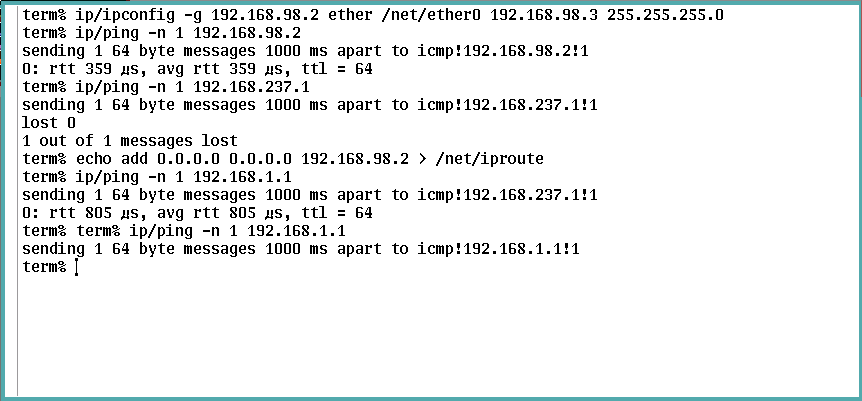
\includegraphics[scale=.5]{ipconfig.png}
\end{figure}

\section{Mise en place de services sur la passerelle}
Par manque de temps, cette section est incomplète par rapport
à ce qui a été fait sur la passerelle Linux en cours. Néamoins,
la configuration est à quelques détails près la même dans
les deux cas. Seule la gestion du routage/firewall change vraiment,
puisque les logiciels utilisés sont dans les deux cas identiques.

\section{Accès distants sur la passerelle}
\subsection{Telnetd}
On utilise inetd pour activer le serveur telnetd automatiquement,
et on s'assure qu'inetd est bien lancé au démmarage de la machine:
\begin{verbatim}
(passerelle)# ed /etc/inetd.conf 
5014
/tel
#telnet stream  tcp     nowait  root    /usr/libexec/telnetd    telnetd
s/^#/
telnet  stream  tcp     nowait  root    /usr/libexec/telnetd    telnetd
wq
5013
(passerelle)# cat >> /etc/rc.conf 
inetd_enable="YES"
^D
(passerelle)# /etc/rc.d/inetd start
Starting inetd.
(passerelle)# echo 'Welcome!' > /etc/motd
\end{verbatim}

On teste que cela marche bien depuis le client:
\begin{figure}[!ht]
	\centering
	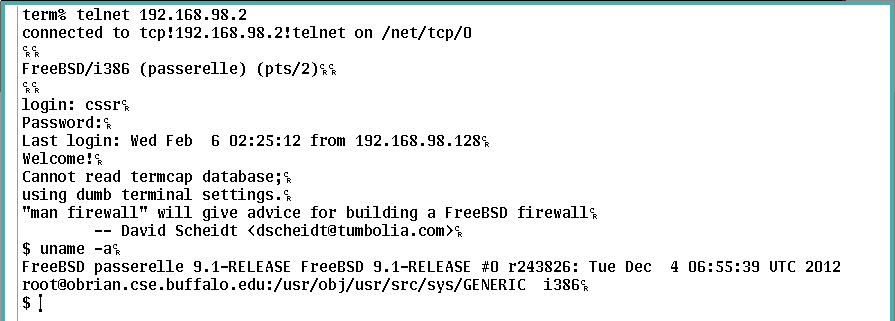
\includegraphics[scale=.5]{telnet.png}
\end{figure}

Comme les paquets passent par des interfaces virtuelles, on
peut les observer depuis la machine hôte sans avoir à se
mettre en homme du milieu. On se reconnecte avec wireshark
démarré sur l'hôte:
\begin{figure}[!ht]
	\centering
	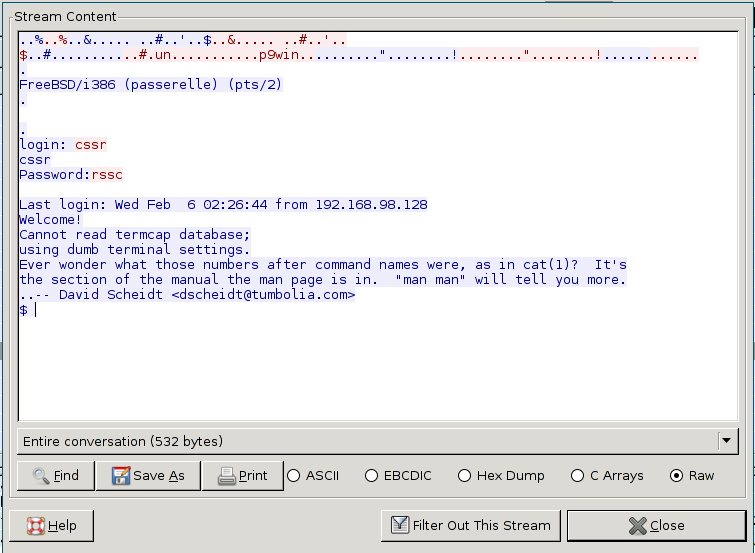
\includegraphics[scale=.5]{telnetsniff.png}
\end{figure}

\subsection{OpenSSH}
À l'installation, il avait été choisi de l'activer par défaut. On
s'assure que c'est bien le cas:
\begin{verbatim}
(passerelle)# grep ssh /etc/rc.conf 
sshd_enable="YES"
\end{verbatim}

% http://plan9.bell-labs.com/wiki/plan9/ssh_configuration/
Le client ssh plan9 ne fonctionne qu'avec la version $1$ du
protocole (une version incomplète de la version $2$ est
disponibles dans \textit{/n/contrib/blstuart/ssh}). On modifie
donc la version du protocole, et on redémarre le service:
\begin{verbatim}
(passerelle)# grep Protocol /etc/ssh/sshd_config
Protocol 1
(passerelle)# /etc/rc.d/sshd restart
Stopping sshd.
Starting sshd.
\end{verbatim}

Côté client, on génère une clef RSA que l'on convertie ensuite
au format requis pour ssh, puis on copie cette version sur la
passerelle via une connection telnet, et enfin, on donne la
clef au gestionnaire de clefs du client (factotum):
\begin{figure}[!ht]
	\centering
	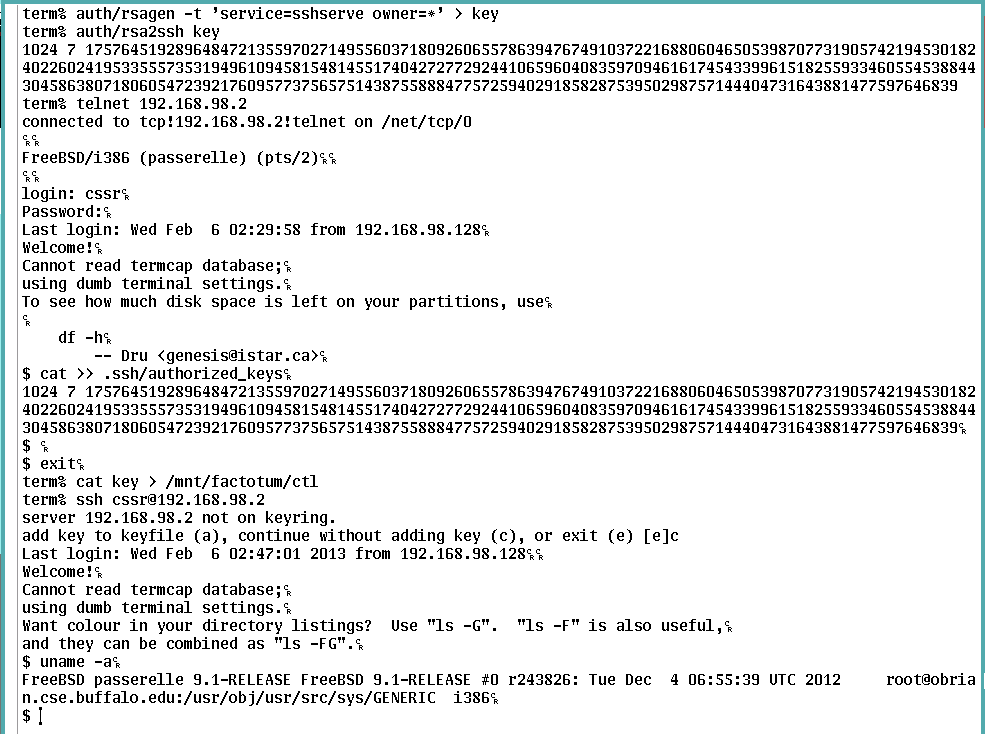
\includegraphics[scale=.5]{sshv1.png}
\end{figure}

\subsection{Nmap}
On inspecte la passerelle depuis le système hôte:
\begin{verbatim}
(host)# nmap -A 192.168.98.2

Starting Nmap 6.25 ( http://nmap.org ) at 2013-02-06 04:24 CET
Nmap scan report for 192.168.98.2
Host is up (0.0011s latency).
Not shown: 998 closed ports
PORT   STATE SERVICE VERSION
22/tcp open  ssh     OpenSSH 5.8p2_hpn13v11 (FreeBSD 20110503; protocol 2.0)
| ssh-hostkey: 1024 ad:53:43:8e:1e:9a:25:59:ef:d7:16:99:d1:21:47:a0 (DSA)
| 2048 ab:d7:19:4c:99:73:6e:f3:0b:ba:56:95:1e:67:92:6d (RSA)
|_256 8a:e1:0c:ab:21:3e:14:4b:74:f4:95:0d:02:f0:21:d3 (ECDSA)
23/tcp open  telnet  BSD-derived telnetd
MAC Address: 00:0C:29:A7:72:B4 (VMware)
Device type: general purpose
Running: FreeBSD 7.X|8.X|9.X|10.X
OS CPE: cpe:/o:freebsd:freebsd:7 cpe:/o:freebsd:freebsd:8 cpe:/o:freebsd:freebsd:9 cpe:/o:freebsd:freebsd:10
OS details: FreeBSD 7.0-RELEASE-p1 - 10.0-CURRENT
Network Distance: 1 hop
Service Info: OS: FreeBSD; CPE: cpe:/o:freebsd:freebsd

TRACEROUTE
HOP RTT     ADDRESS
1   1.10 ms 192.168.98.2

OS and Service detection performed. Please report any incorrect results at http://nmap.org/submit/ .
Nmap done: 1 IP address (1 host up) scanned in 9.31 seconds
\end{verbatim}

\subsection{Génération d'un certificat $X509$}
OpenSSL est déjà installé par défaut; on s'en assure, puis on génère
dans l'ordre:
\begin{enumerate}
	\item une cléf privée;
	\item un CSR (Certificate Signing Request);
	\item un certificat $X509$.
\end{enumerate}

Enfin, on copie (arbitrairement) ces fichiers dans \textit{/etc/ssl/}:
\begin{verbatim}
(passerelle)# openssl version
OpenSSL 0.9.8x 10 May 2012
(passerelle)# openssl req -new -key ca.key -out ca.csr
You are about to be asked to enter information that will be incorporated
into your certificate request.
What you are about to enter is what is called a Distinguished Name or a DN.
There are quite a few fields but you can leave some blank
For some fields there will be a default value,
If you enter '.', the field will be left blank.
-----
Country Name (2 letter code) [AU]:FR
State or Province Name (full name) [Some-State]:France
Locality Name (eg, city) []:Nice
Organization Name (eg, company) [Internet Widgits Pty Ltd]:CSSR Ltd
Organizational Unit Name (eg, section) []:
Common Name (e.g. server FQDN or YOUR name) []:
Email Address []:

Please enter the following 'extra' attributes
to be sent with your certificate request
A challenge password []:A challenge password
An optional company name []:
(passerelle)# openssl x509 -req -days 365 -in ca.csr -signkey ca.key -out ca.crt
Signature ok
subject=/C=FR/ST=France/L=Nice/O=CSSR Ltd
Getting Private key
(passerelle)# cp ca.* /etc/ssl/
\end{verbatim}

Le certificat pourra être utilisé par les serveurs HTTPS, SMTP, IMAPS, etc.

\subsection{HTTPs}
